% nn-6b.png -- the MLP of section 3.6 (multiLayerRegression(1, 5, 3, 1)).
% The data has a single feature, so the input is drawn in the collapsed
% (vector) form introduced by the nn-5 pair.
% Build: bash tools/figures/build.sh
\documentclass[tikz,border=5pt]{standalone}
% Shared style for the neural-network diagrams in notebooks/img/nn-*.png.
% Palette and look are matched to the pre-existing figures (nn-1..nn-8,
% backprop-*) so a regenerated figure sits next to them unnoticed.
\usepackage[T1]{fontenc}
\usepackage{newtxtext}
\usepackage{newtxmath}
\usetikzlibrary{arrows.meta,calc,positioning}

\definecolor{innavy}{HTML}{004475}     % input neurons, source-like labels
\definecolor{hidyellow}{HTML}{FFCF6E}  % hidden neurons
\definecolor{outmaroon}{HTML}{8E1854}  % output neuron
\definecolor{accgold}{HTML}{E5A600}    % "Hidden Layer" label
\definecolor{gridgrey}{HTML}{B7B7B7}

\tikzset{
  neuron/.style   = {circle, draw=black, line width=0.9pt, minimum size=0.9cm,
                     inner sep=0pt, font=\large\bfseries},
  hidden/.style   = {neuron, fill=hidyellow},
  inputn/.style   = {neuron, fill=innavy, text=white},
  outputn/.style  = {neuron, fill=outmaroon, text=white},
  conn/.style     = {-{Latex[length=2.2mm,width=1.6mm]}, line width=0.7pt},
  bias/.style     = {-{Latex[length=1.8mm,width=1.3mm]}, line width=0.7pt},
  biaslbl/.style  = {font=\scriptsize, inner sep=1pt},
  layerlbl/.style = {font=\large\bfseries},
}

% Column positions shared by every figure (1 unit = 1cm).
\def\HIDX{3.4}   % hidden neurons
\def\ACTX{4.9}   % activation insets (centre)
\def\OUTX{7.4}   % output neuron
\def\NODE{0.45}  % neuron radius
\def\BOX{0.42}   % activation inset half-width

% Framed mini-plot of the sigmoid, drawn where the existing figures draw it.
% Usage: \actinset{x}{y}{label}
\newcommand{\actinset}[3]{%
  \begin{scope}[shift={(#1,#2)}]
    \fill[white] (-\BOX,-\BOX) rectangle (\BOX,\BOX);
    \foreach \g in {-0.14,0.14}{%
      \draw[gridgrey, line width=0.35pt] (-\BOX,\g) -- (\BOX,\g);
      \draw[gridgrey, line width=0.35pt] (\g,-\BOX) -- (\g,\BOX);}
    \draw[black, line width=1.1pt, domain=-0.40:0.40, samples=60]
      plot ({\x}, {0.78/(1+exp(-9*\x)) - 0.39});
    \draw[black, line width=0.9pt] (-\BOX,-\BOX) rectangle (\BOX,\BOX);
    \node[above left, font=\scriptsize, inner sep=1pt] at (\BOX,\BOX+0.02) {#3};
  \end{scope}}

% Bias arrow plus label above a neuron: \biasup{node name}
\newcommand{\biasup}[1]{%
  \draw[bias] ($(#1)+(0,\NODE+0.41)$) -- ($(#1)+(0,\NODE+0.01)$);
  \node[biaslbl, above] at ($(#1)+(0,\NODE+0.41)$) {Bias};}

% A vector collapsed into one node: two offset discs behind it.
% Usage: \vectornode{x}{y}{label}
\newcommand{\vectornode}[3]{%
  \foreach \dx/\dy in {0.13/0.11, 0.26/0.22}{%
    \draw[innavy, line width=0.7pt, fill=innavy!22]
      ($(#1,#2)+(\dx,\dy)$) circle (\NODE);}
  \node[inputn] (#3) at (#1,#2) {$#3$};}

\begin{document}
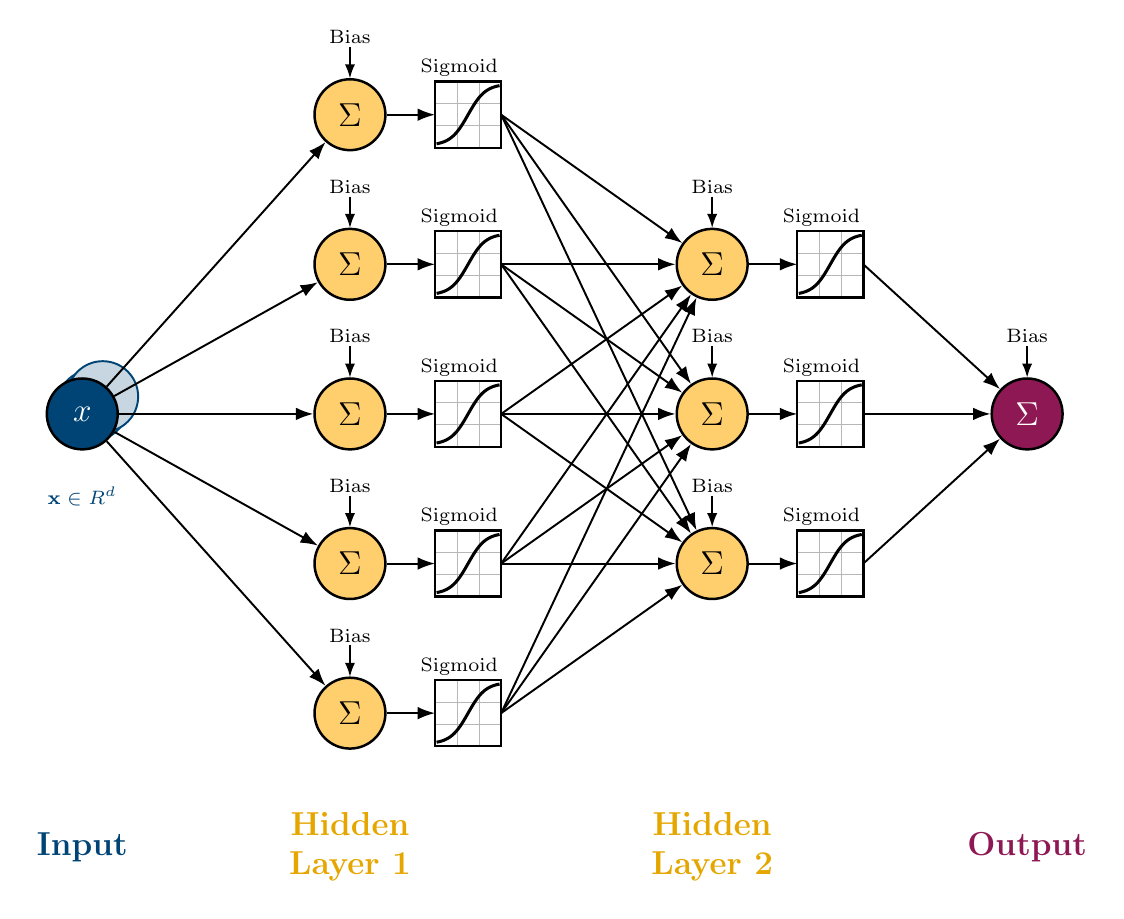
\begin{tikzpicture}[x=1cm,y=1cm]

\def\HIDAX{3.4}
\def\ACTAX{4.9}
\def\HIDBX{8.0}
\def\ACTBX{9.5}
\def\OUTBX{12.0}

\vectornode{0}{0}{x}
\node[font=\scriptsize, text=innavy] at (0,-1.05) {$\mathbf{x}\in\mathbb{R}^{d}$};

\foreach \j/\yy in {1/3.8, 2/1.9, 3/0.0, 4/-1.9, 5/-3.8}{
  \node[hidden] (a\j) at (\HIDAX,\yy) {$\Sigma$};
  \actinset{\ACTAX}{\yy}{Sigmoid}
  \draw[conn] (a\j) -- (\ACTAX-\BOX,\yy);
  \biasup{a\j}}

\foreach \j/\yy in {1/1.9, 2/0.0, 3/-1.9}{
  \node[hidden] (b\j) at (\HIDBX,\yy) {$\Sigma$};
  \actinset{\ACTBX}{\yy}{Sigmoid}
  \draw[conn] (b\j) -- (\ACTBX-\BOX,\yy);
  \biasup{b\j}}

\node[outputn] (o1) at (\OUTBX,0) {$\Sigma$};
\biasup{o1}

\foreach \j in {1,...,5}{\draw[conn] (x) -- (a\j);}
\foreach \yy in {3.8,1.9,0.0,-1.9,-3.8}{%
  \foreach \j in {1,2,3}{\draw[conn] (\ACTAX+\BOX,\yy) -- (b\j);}}
\foreach \yy in {1.9,0.0,-1.9}{\draw[conn] (\ACTBX+\BOX,\yy) -- (o1);}

\node[layerlbl, text=innavy,    align=center] at (0,-5.5)      {Input};
\node[layerlbl, text=accgold,   align=center] at (\HIDAX,-5.5) {Hidden\\Layer 1};
\node[layerlbl, text=accgold,   align=center] at (\HIDBX,-5.5) {Hidden\\Layer 2};
\node[layerlbl, text=outmaroon, align=center] at (\OUTBX,-5.5) {Output};

\end{tikzpicture}
\end{document}
